
\section{Introduction}
    \subsection{Background}
        The Norwegian electrical grid is almost exclusively provided by power generated by hydro electric power plants \cite{Energi212014}. Many of the biggest power plants have been producing power for over five decades \cite{vannkraft}, and many of them are in need of upgrades \cite{tu}. Hydro electric power plants are now and then stopped for maintenance. This is in some cases of course unavoidable, since all equipment has a certain life span, and hence needs replacement, but in many cases components are overhauled and changed without showing signs of wear and or damage. 
        
        
        
        
    \subsection{Motivation}
    
        Two important factors in a hydro electric power-plant follow. Firstly, it is important that all the rainwater collected is used to produce power. This means that having reservoirs so full that they flood over is like throwing money into the river. Secondly as with all power plants, you want to produce most of your power when the prices are as high as possible. This can be solved by keeping the plants power production, and hence water usage at optimal levels at all time. This again means that you can optimize your production, as long as your plant is operable. Another important factor is the fact that hydro electric power is a clean power source. In a world that desperately needs clean power, every little improvement is welcome addition. 
        
        
    \subsection{Problem definition}    
        In hydro electric power plants today, there is little to no condition estimations. Maintenance is scheduled based on running hours, planned maintenance or break downs. This project looks into condition monitoring for a very specific part of a hydro electric power plant, the dead band of the guide vanes for a Francis turbine. The guide vanes are what controls  how much water is led onto the turbine at any given time. These guide vanes are controlled by one or two hydraulic motors, through a series of mechanical components. Figure \ref{fig:servo_plant} shows such a servo motor controlling the guide vanes. As a turbine system ages, the dead band of the guide vanes increase. The dead band explains how much differential force is need to change the direction of motion of the guide vanes, from opening to closing or closing to opening. This can be compared to the dead band found in valves \cite{Choudhury2005}. The dead band is connected to the friction coefficient of the guide vanes. As the guide vanes are worn down, the friction increases, and so does the dead band.  
        
        % \begin{figure}
        %     \begin{minipage}[b]{0.5\linewidth}
        %         \centering
        %         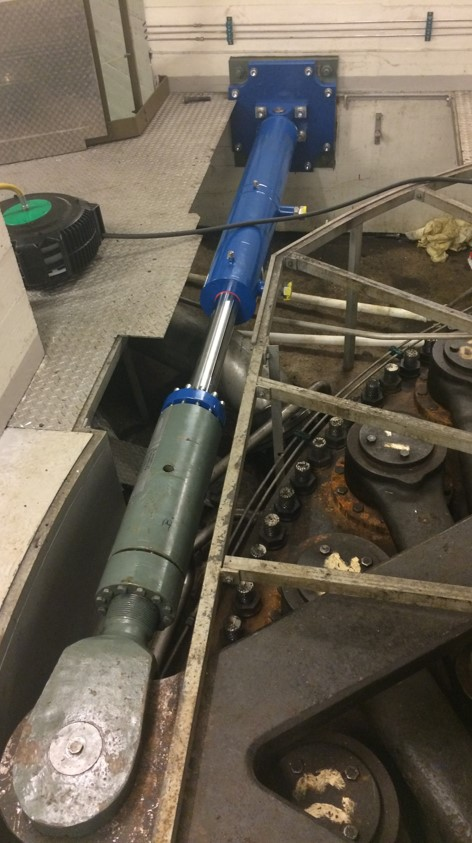
\includegraphics[scale = 0.5]{figures/introduction/servo1.jpg}
        %         \caption{Servo motor for either closing or opening at an actual plant. It is connected to a ring which controls the opening of the guide vanes. Courtesy of Hymatek Controls.}
        %         \label{fig:servo_plant}
        %     \end{minipage}
        %     \hfill
        %     \begin{minipage}[b]{0.5\linewidth}
        %         \centering
        %         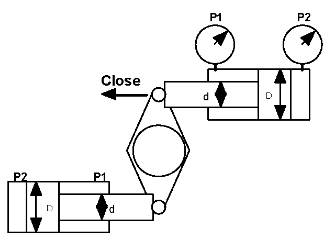
\includegraphics[scale = 0.5]{figures/introduction/servo.png}
        %         \caption{Schematic showing the how the opening and closing servos act upon the system.}
        %         \label{fig:servo_schematic}
        %     \end{minipage}
        % \end{figure}
    
        \begin{figure}
            \centering    
            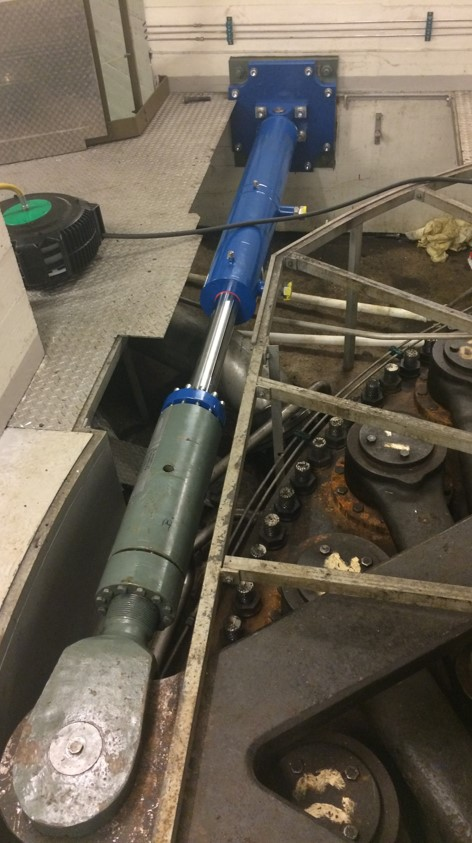
\includegraphics[scale = 0.5]{figures/introduction/servo1.jpg}
            \caption{Servo motor for either closing or opening at an actual plant. It is connected to a ring which controls the opening of the guide vanes. Courtesy of Hymatek Controls.}
            \label{fig:servo_plant}
        \end{figure}
        When the friction becomes too large, the hydraulic system will not be able to control the system as wanted. Today the condition of the guide vanes and its mechanical components are found by disconnecting the generator from the grid, and performing a servo indication. By disconnecting the generator from the grid the water flow over the turbine can be manipulated without having to worry about output voltage and frequency. It is crucial that the procedure is performed so slowly that the footprint of the water power is negligible. 
        
        When a generator is delivering power to the grid, wast amounts of water are flowing through the system at any given time. The guide vanes are adjusted with respect to the power the generator is delivering to the grid. Changes in the restriction of water flow (change of guide vane position) can generate disturbances and overshoot in the system. This can be spotted as noise in the measured process signals. When a servo indication is performed, the rate of change of water restriction (changing of the guide vanes position) is so slow that the effects from the water are minimized. This gives much cleaner process signals, that are easier to analyze, because they mostly consist of data relevant to the dead band estimation.
        
        However if it could be possible to create an estimate of the dead band and hence the friction coefficient during normal operation, this would be very beneficial. Firstly this will reduce costs. Today the analysis are outsourced to consultants, and they need to mount new equipment to take the necessary measurements. This again leads to increased plant activity. Secondly, downtime due to an hour based maintenance schedule, can be reduced. Finally, it introduces a constant estimate of the condition of the plant, something that is not available today. This is however not a straight forward thing to solve. To begin, creating a classifier which enables detection of changes in the condition of the guide vanes is a natural first step. This is the focus of the project. The guide vane friction issue is similar to problems found in valves. According to \cite{Dozat} there is a clear need for methods to detect and quantify the stiction in valves. Hence, if one can find a solution to estimating the condition of the guide vanes, this might be applicable to the process industry as well. 
        
        
    \subsection{The techniques used}    
        Building a model for the dead band of the guide vanes is complex. There can be complex hysteresis effects, and the shape of the curve can be very nonlinear. An example of the deadband of a guide vane system is shown in Figure \ref{fig:deadband}. There are even worse cases where the "banana" shape becomes even steeper and narrower at the ends. These nonlinearities makes it hard to create a general model. Each turbine has its own maintenance schedule, and they might not have the same mechanical components. This means that a model that works great for one system, might not be valid at all for another. Therefore, it has been chosen to focus on databased methods, to try to create a classifier for the condition of the guide vanes. These can be trained on measurements taken from each individual turbine, reducing the time and cost compared to creating a mathematical model for each. 
        
        \begin{figure}
            \centering
            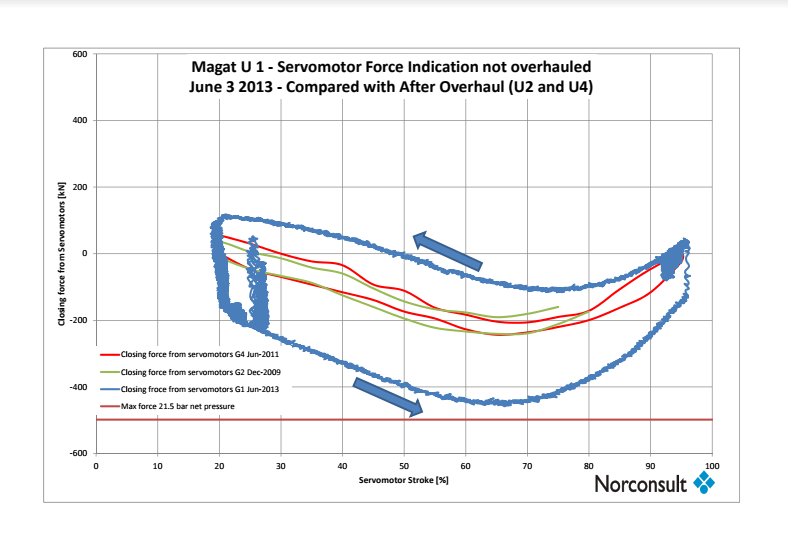
\includegraphics[width=0.8\textwidth]{figures/introduction/deadband.png}
            \caption{Deadband of servoindication, courtesy of Norconsult}
            \label{fig:deadband}
        \end{figure}

        As for the data based methods, three separate methods have been chosen. Most importantly because they span machine learning from simple to advanced. If the problem can be solved using a simple method, there is no need to use a more complex one. Also, the simpler machine learning methods are the ones easiest to interpret in how they separate the data. For this project, logistic regression, support vector machines and neural networks are the methods chosen. Each of them will be tested and compared to one another. 
        
    \subsection{Case studies}   
        As mentioned in the motivation section, this project looks into condition monitoring of the guide vanes found in a Francis generator. The data available for analysis comes from four similar generator sets, with different running hours since last overhaul. This means that the four different data sets, can be viewed as coming from the same generator over many years. Hence these four cases, can be used to create classifiers that can classify the condition of the generator into four different classes, from good to bad. The datasets consist of a series of time-series data samples stored in a series of .csv files. These time-series are taken during commissioning and servo indication. %Figure \ref{fig:data} shows the different variables found in the data set.
        
        Today the servo indications are manually analyzed by engineers. Hence enabling automatic classification based on a servo indication measurement will be a step forward. This is the first case looked into. One servo indication dataset is available for each of the four generators. The first task is then to create a classifier that based on the servo indications are able classify the condition of the guide vanes into four different categories. Notice that here only classification is looked into, it is not made an attempt to estimate the actual level of friction in the guide vanes.
        
        The second task, is trying to recreate similar classifiers, based on measurements taken during commissioning of the same generators. These measurements include disturbances and might be more difficult to analyze than the pure servo indication data. If it could be shown possible to find dead band information from these noisy data measurements, this is a step towards enabling real time assessment of the condition of the guide vanes, and remove the need for taking servo indications.

        % Insert image of the four different cases. 
        
        % \begin{figure}
        %     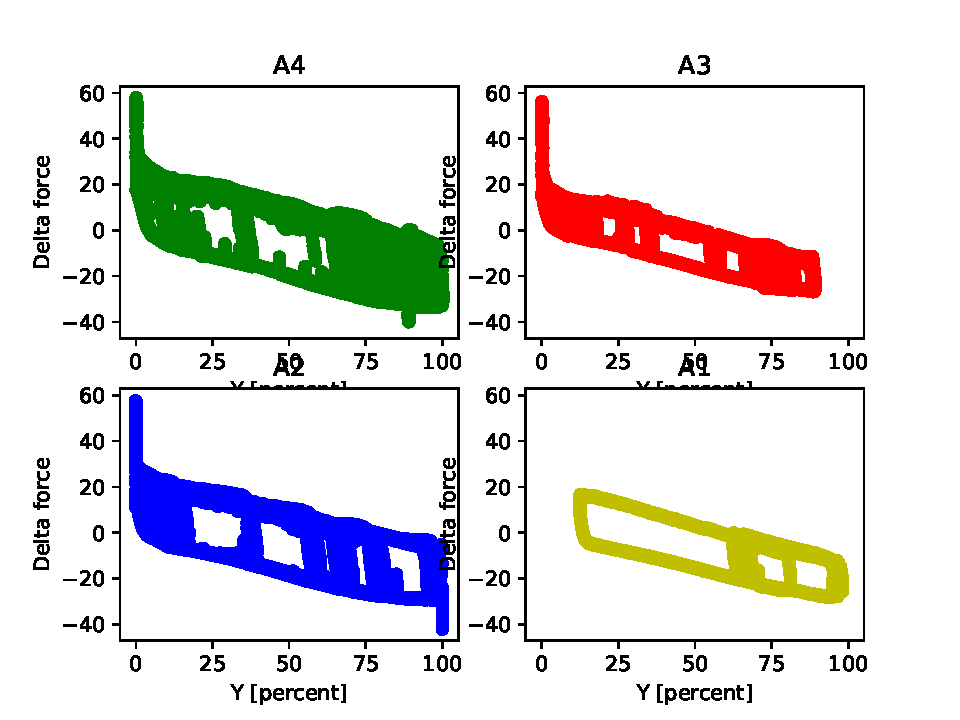
\includegraphics[width=\textwidth]{figures/introduction/ServoIndicationsub.pdf}
        %     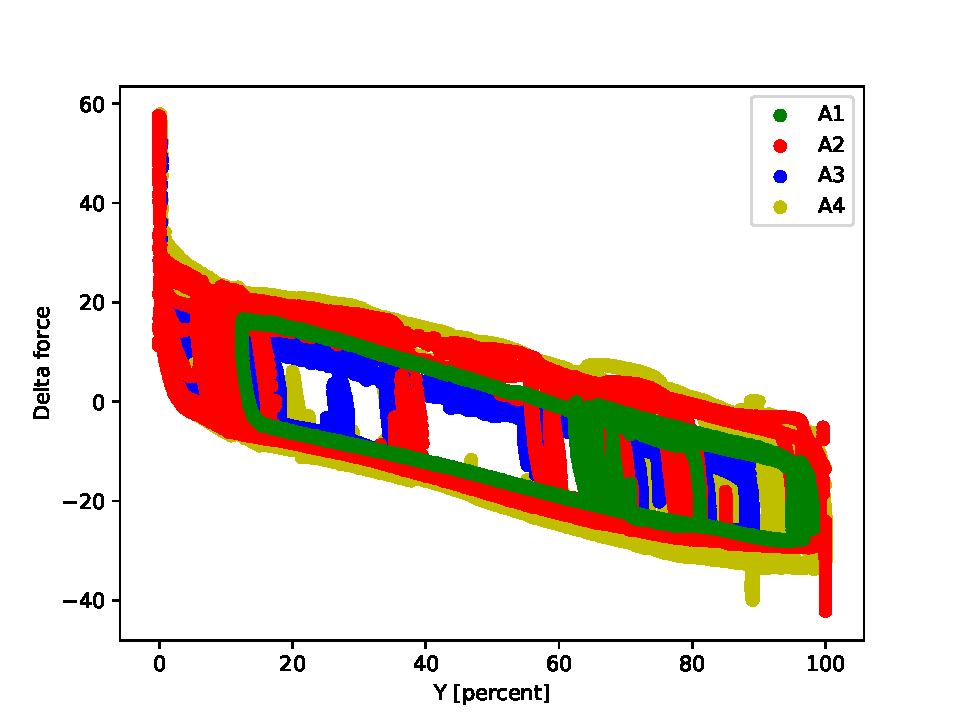
\includegraphics[width=\textwidth]{figures/introduction/ServoIndication.pdf}
        % \end{figure}
        
        
        
        
        
    % \subsection{Literary analysis}
    
    %     overordna, condition monitoring
    %     hydropower
    %     cm on hydraulics?
    %     State of the art of condition monitoring of hydraulics at the moment? 
        
        

